\documentclass[letterpaper, 11pt]{article}
\usepackage[inner = 0.75in, outer = 0.75in, top = 1in, bottom = 1in, bindingoffset = 0.0 cm]{geometry}
\usepackage{amsmath}	% provides enhancement of math printout structure 
\usepackage{amssymb}	% provides an extended symbol collection
\usepackage{comment}	% package to use comment block
\usepackage{sectsty}	% to change the style of section headers
\usepackage{fancyhdr}	% to have fancy headers for each page
\usepackage{graphicx}	% allows you to import images
\usepackage{float}	% allows the control of float positions
\usepackage{makeidx} 	% to create index pages
\makeindex

% List of macros
\newcommand{\fourier}[2]{\mathcal{F}_{#1}[#2]} % Fourier transform notation
\newcommand{\fint}{\int_{-\infty}^{\infty}} % integral with infinite limits
\newcommand{\ft}[3]{\fint #2 e^{-2\pi i#3#1} d#1} % Fourier transform 
\newcommand{\ift}[3]{\fint #2 e^{2\pi i#1#3} d#1} % Inverse Fourier transform 
\newcommand{\sed}[2]{#2_{0}e^{2\pi if_{0}#1}e^{-#1/T} \theta (#1)} % SED function
\newcommand{\fsum}[1]{\sum_{#1 = -\infty}^{\infty}}
\newcommand{\spf}[2]{\Delta #1 \fsum{#2} \delta (#1 - #2 \Delta #1)}
% Numbering equation and figure with section number
\numberwithin{equation}{section}
\numberwithin{figure}{section}

% Centering section titles
\sectionfont{\centering}

\begin{document}
% Front cover page with title and name
\begin{titlepage}
	\begin{center}
		% \vfill must have preceding text line
		\Huge{\bfseries Fourier Transform}\vfill 
	\end{center}

	\begin{flushright}
		Sejin Nam\\
		University of Hawaii at Manoa
	\end{flushright}
\end{titlepage}

\begin{comment} % commenting out standard title page
\title{Fourier Transform}
\author{Sejin Nam}
\date{May 20}
\maketitle
\thispagestyle{empty}
\clearpage
\end{comment}

% page numbering in roman numerals
\pagenumbering{roman}

% Preface
\section*{\centering Preface}
Fourier transform is a mathematical transformation, in the context of my exposition, that maps one function in time domain into another function in frequency domain. There are two types of FT, Fourier transform in short: continuous and discrete. Discrete FT is of great importance in many modern data processing application as modern computers are digital, meaning they perform computation in discrete manner. In this article, I'll discuss a continous case first before moving onto the discrete case.
\cleardoublepage

% Table of Contents
\tableofcontents
\clearpage

% use fancyhdr
\pagestyle{fancy}

% First Section: prerequisite mathematics
\pagenumbering{arabic}
\section{Prerequisite Mathematics}
A few prerequisite mathematics will be discussed here first in anticipation of their requirements in the discussion of subsequent sections of Fourier transform. In this article, it is implied that all the functions discussed are \(\mathbb{R} \mapsto \mathbb{C} \), infinitely differentiable, and absolutely integrable unless stated otherwise.  

% 1.1 Dirac Delta Function
\subsection{Dirac Delta Function}\index{Dirac Delta function}
The Dirac Delta function, \(\delta (t)\), has the following property:
\begin{align}
	\delta (t)	&=\begin{cases}
		\infty, & \text{if } t = 0 \\
		0,	& \text{otherwise}
	\end{cases}\\
		1	&= \fint \delta (t) dt
\end{align}
(In my discussion of function, \(t\) variable represents time physically). The following integral is also the Dirac Delta function:
\begin{align}
	\delta (t)	&= \ift{f}{}{t}\label{eq:dirac}
\end{align}
The above relations will be used throughout the discussion of this article.

% 1.2 Sinusoidal expoential decay function
\subsection{Sinusoidal exponential decay function}\index{SED}
Sinusoidal exponential decay function (I call it SED) is as follows:
\begin{equation}
	\begin{aligned}[b]
		x &= x_{0}\cos{(2\pi f_{0}t)}e^{-t/T} \theta(t)
		\label{eq:rsed}
	\end{aligned}
\end{equation}
Where \(\theta (t)\) is a Heaviside step function (the plot of such function is given in figure \ref{fig1}). You can have sine instead of cosine in the above expression. For our discussion, SED of choice is combination of sine and cosine exponential decays in complex form:
\begin{equation}
	\begin{aligned}[b]
		x	&= x_{0}\cos{(2\pi f_{0}t)}e^{-t/T} \theta(t)+ i x_{0}\sin{(2\pi f_{0}t)}e^{-t/T} \theta(t)\\
			&= (\cos{(2\pi f_{0}t)} +i \sin{(2\pi f_{0}t)})x_{0}e^{-t/T} \theta(t) \\
			&= \sed{t}{x}
			\label{eq:sed}
	\end{aligned}
\end{equation}
The real part of \eqref{eq:sed} is simply \eqref{eq:rsed}.

% 1.3 Sampling function  
\subsection{Sampling function}\index{Sampling function}
The sampling function, denoted as \(u(t)\), with the sampling interval \(\Delta t\) is as follows:
\begin{equation}
	\begin{aligned}[b]
		u(t) = \spf{t}{n}
	\end{aligned}
\end{equation}
The function is periodic with the period being the sampling interval. 

% figure for sed function
\begin{figure}[H]
	\centering
	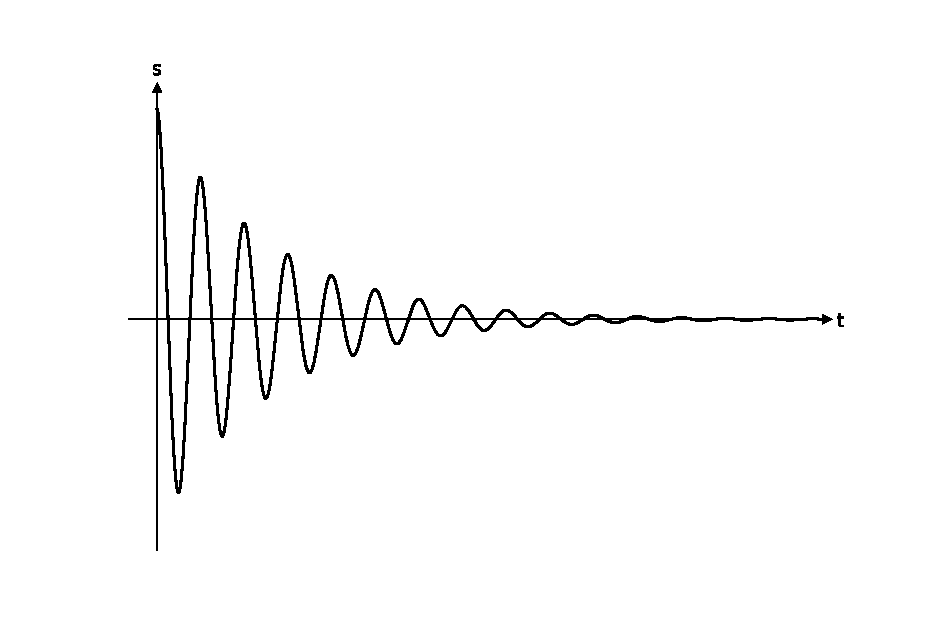
\includegraphics[height=5in]{sed.eps}
	\caption{sed function plot, s vs. t}
	\label{fig1}
\end{figure}


\clearpage
% Second Section: Continuou Fourier transform
\section{Continuous Fourier Transform}\index{Fourier transform}

% 2.1 Definition of Fourier transform
\subsection{Definition of Fourier transform}
Consider a continuous function of \(t\), \(x(t)\). The continuous FT of \(x\), \(X(f)\), is as follows:
\begin{equation}
	\begin{aligned}[b]
		X(f)	&=\fourier{t}{x} \\
			&=\ft{t}{x(t)}{f}
	\end{aligned}
\end{equation}
\(X(f)\) is also continuous in \(f\) (in my discussion \(t\) and \(f\) represent time and frequency respectively). \(\fourier{t}{x}(f)\) notation can be used to explicitly indicate that \(x\) is transformed into \(f\) domain. It is easy to see that if \(a\) is a constant, then \(\fourier{t}{ax} = a \fourier{t}{x}\). You can also perform inverse FT on \(X\), which is:
\begin{equation}
	\begin{aligned}[b]
		\fourier{f}{X}	&= \ift{f}{X(f)}{t} \\
				&= \ift{f}{\left ( \ft{\tau}{x(\tau)}{f}\right )}{t} \\
				&= \fint x(\tau) \fint e^{2\pi if(t - \tau)} df d\tau \\
				&= \fint x(\tau) \delta (t - \tau) d\tau \\
				&= x(t)
	\end{aligned}
\end{equation}
where I used \eqref{eq:dirac} orthogonality relation (We will continue to use the notation \(x(t)\) and \(X(f)\) as an example of FT pair throughout the discussion). It is also easy to see that the inverse FT of one is the Dirac Delta function.

% 2.2 FT with the extra phase factor
\subsection{FT with the extra phase factor}
Consider another function, \(e^{2\pi i f_{0} t}x(t)\). The FT of it is:
\begin{equation}
	\begin{aligned}[b]
		\fourier{t}{e^{2\pi i f_{0} t}x(t)}
			&= \ft{t}{e^{2\pi i f_{0} t}x(t)}{f}\\
			&= \ft{t}{x(t)}{(f - f_{0})}\\
			&= \fourier{t}{x}(f - f_{0})\\
			&= X(f - f_{0})
	\end{aligned}
\end{equation}
It is simply the FT of \(x\) in \(f - f_{0}\) in domain.

% 2.3 Sinusoidal exponential decay signal \subsubsection{Sinusoidal exponential decay function} Sinusoidal exponential decay (I call it SED) function is as follows:
\subsection{FT of SED}
Consider a SED function discussed before, \(x = \sed{t}{x}\). The FT of \(x\) is (with \(1/T = r\)) as follows:
\begin{equation}
	\begin{aligned}[b]
		X(f)	&= \fourier{t}{x}\\
			&= \fourier{t}{\sed{t}{x}}\\
			&= s_{0}\fourier{t}{e^{-rt} \theta (t)}(f - f_{0})\\
			&= \frac{s_{0}}{r + 2\pi i(f - f_{0})} \\
			\gdef\temp{r^2 + 4\pi^{2}(f - f_{0})^2} % temporary macro
			&= s_{0}\frac{r - 2\pi i(f - f_{0})}{\temp}\\
			&= s_{0}\left[\frac{r}{\temp} + i\frac{2\pi(f_{0} - f)}{\temp} \right]
	\end{aligned}
\end{equation}

% 2.4 FT of the sampling function
\subsection{FT of the sampling function}
Suppose \(u(t)\) is the sampling function with the sampling interval \(\Delta t\). Then the FT of \(u\) is:
\begin{equation}
	\begin{aligned}[b]
		\fourier{f}{u}
			&= \ft{t}{u(t)}{f} \\
			&= \ft{t}{\spf{t}{n}}{f} \\
			&= \Delta t \fsum{n} e^{-2\pi ifn\Delta t} \fint \delta (t - n \Delta t) dt \\
			&= \Delta t \fsum{n} e^{-2\pi ifn\Delta t}
	\end{aligned}
\end{equation}

\printindex
\end{document}
